\documentclass{article}

\usepackage[utf8]{inputenc}
\usepackage[greek,english]{babel}
\usepackage{alphabeta}
\usepackage{pgfplots}
\usepackage{amsmath}
\graphicspath{ {./images/} } % ο φάκελος που έχω τις εικόνες για τα γραφήματα
\pgfplotsset{compat=1.18} % για κάποιο λόγο είχα ένα warning και το overleaf πρότεινε να προσθέσω αυτό

\title{Πρώτη Εργασία Στο Μάθημα της Αριθμητικής Ανάλυσης}
\author{Ονοματεπώνυμο: Σταύρος Νικολαΐδης  \\  ΑΕΜ: 3975}
\date{Δεκέμβριος 2021}

\begin{document}


\maketitle

\section{Πρώτη Άσκηση}

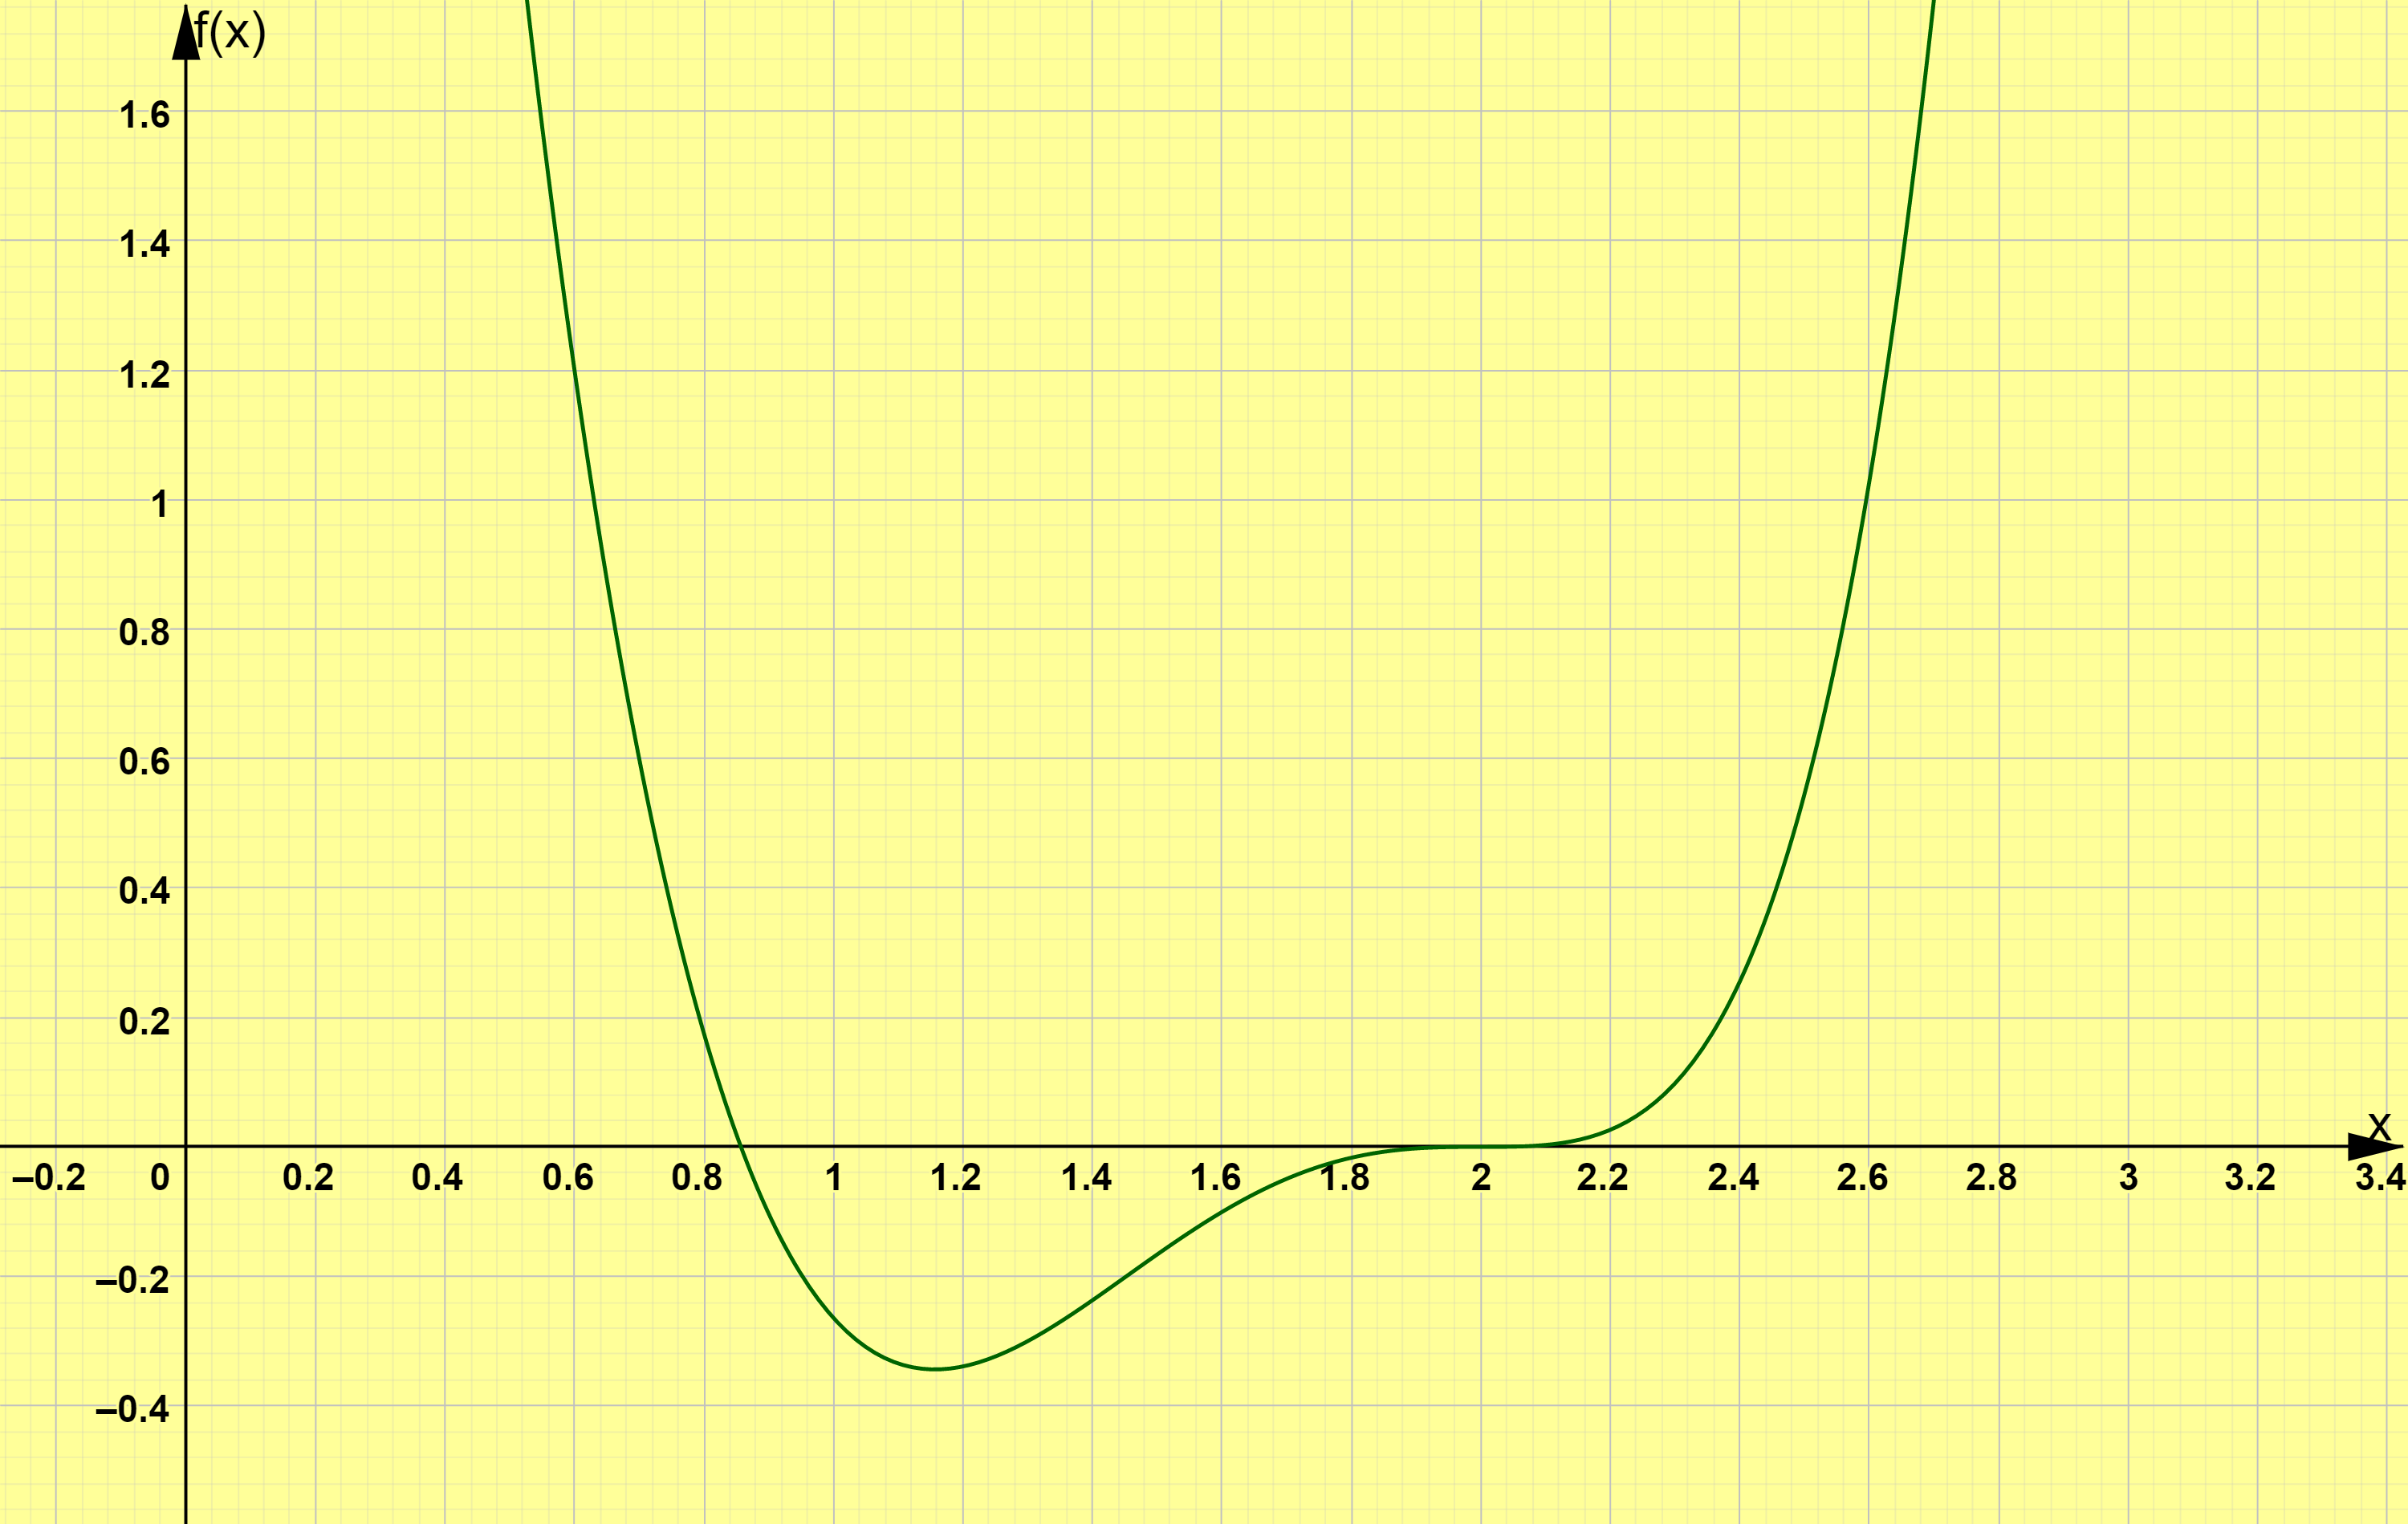
\includegraphics[width=12cm, height=8cm]{images/Figure_1.png} \\
Γραφική παράσταση της συνάρτησης: \( f(x) = 14xe^{x-2} - 12e^{x-2} - 7x^3 + 20x^2 - 26x + 12 \)

\vspace{5mm} 
\large{\underline{Μερικά γενικά για την συνάρτηση: }} \\
Όπως παρατηρούμαι η συνάρτηση είναι τρίτου βαθμού επομένως περιμένουμε να έχει το πολύ τρεις ρίζες. Αρχικά στην γραφική παράσταση φαίνεται να έχουμε 2 ρίζες, μία κοντά στο 0,8 και μία κοντά στο 2. Θα χρειαστεί να επιβεβαιώσουμε αν κάποια από αυτές είναι διπλή ρίζα.

\vspace{3mm}
\subsection{Μέθοδος της διχοτόμισης: }

Αρχείο κώδικα: "ex 1a.py" \\

Η μέθοδος της διχοτόμισης ψάχνει την ρίζα αναδρομικά σε ένα διάστημα που όλο και μικραίνει (διχοτομείται) χρησιμοποιόντας το μέσο του διαστήματος για να ελέγξει αν αυτό μηδενίζει την συνάρτηση. Σε περίπτωση που δεν την μηδενίζει, δημιουργείται ένα νέο διάστημα Ι: \\

\vspace{3mm}
Αν \(f(a)f(m) < 0\) τότε Ι = (a, m). \\

Αλλιώς αν \(f(a)f(m) \geq 0\) τότε Ι = (m, b). \\

όπου m το μέσο του αρχικού διαστήματος (a, b). \\

\textbf{Σημείωση:} σε κάθε διάστημα I πρέπει να ισχύει το θεώρημα Bolzano ώστε να υπάρχει τουλάχιστον μία ρίζα για να βρει η μέθοδος. \\

Συνθήκη τερματισμού: Η μέθοδος τερματίζει όταν η διαφορά των άκρων του διαστήματος γίνει μικρότερη του σφάλματος ανοχής που στην προκειμένη περίπτωση είναι ίσο με \(ε = \frac{10^{-5}}{2}\). \\

Η μέθοδος της διχοτόμησης έχει μερικά προβλήματα στον υπολογισμό της ριζάς. Αρχικά δεν μπορεί να βρει και τις 2 ρίζες που υπάρχουνε. Επομένως θα κάνουμε χρήση της μεθόδου σε δύο ξεχωριστά διαστήματα, [0, 1.5] και [1.5, 3] ώστε να βρούμε της ρίζες. \\

Με την μέθοδο της διχοτόμισης μπορούμε να ξέρουμε πριν καν τρέξουμε το πρόγραμμα τον μικρότερο αριθμό επαναλήψεων που θα χρειαστούμε για να προσεγγίσουμε την ρίζα εφαρμόζοντας τον εξής τύπο: 

\[n > \frac{\ln(b-a) - \ln(ε)}{\ln(2)}\]

Όπου: n ο αριθμός των επαναλήψεων, a και b τα άκρα του διαστήματος και \(ε = 0.5 * 10^k\), όπου k τα ψηφία για την ακρίβεια που θέλουμε. \\

Επομένως για να προσεγγίσουμε τις 2 ρίζες με ακρίβεια 5 δεκαδικών ψηφίων, που και οι δυο βρίσκονται σε ένα διάστημα με εύρος 1.5, θα χρειαστούμε τουλάχιστον 19 επαναλήψεις. \\

Αποτελέσματα για την πρώτη ρίζα: \\
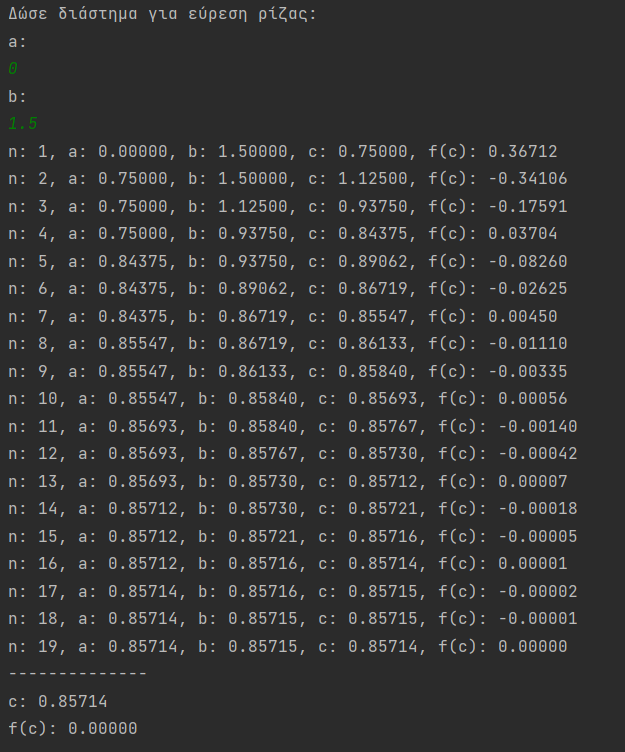
\includegraphics[width=13cm, height=14cm]{images/results_1.png} \\ 
Όπως βλέπουμε η μέθοδος χρειάστηκε 19 επαναλήψεις ώστε να βρει προσεγγιστηκά την πρώτη ρίζα, δηλαδή την 0.85714 στο διάστημα [0, 1.5]. \\ 

Αποτελέσματα για την δεύτερη ρίζα: \\
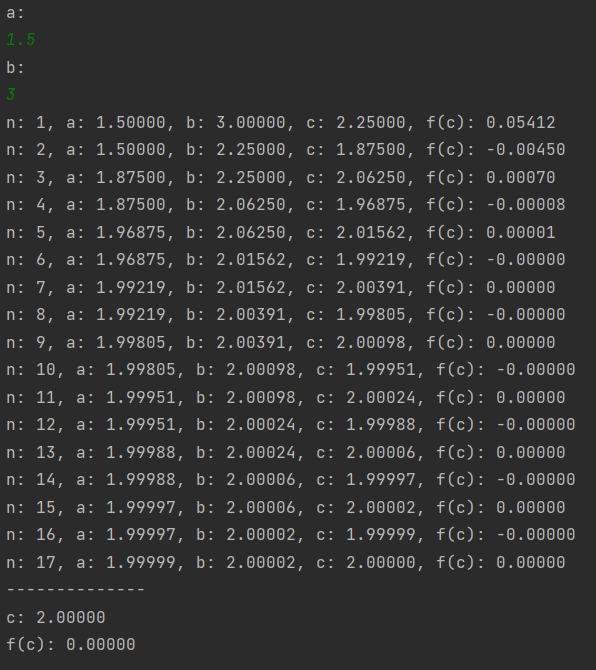
\includegraphics[width=13cm, height=14cm]{images/results_2.png} \\
Όπως βλέπουμε η μέθοδος χρειάστηκε 17 επαναλήψεις ώστε να βρει την δεύτερη ρίζα, δηλαδή την 2. \\ 

\vspace{3mm}
\subsection{Μέθοδος Newton-Raphson: }

Αρχείο κώδικα: "ex 1b.py" \\

Η μέθοδος Newton-Raphson αξιοποιεί την πρώτη παράγωγο της συνάρτησης και μέσω του αναδρομικού τύπου:
\[x^{(k+1)} = x^{(k)} - \frac{f(x^{(k)})}{f'(x^{(k)})} , \hspace{0.5cm} k \geq 0\]
όπου x0 ένα αρχικό σημείο για το οποίο ισχύει: \(f(x_0)*f''(x_0) > 0\), προσεγγίζουμε την ρίζα της εξίσωσης. Η μέθοδος τερματίζει αν η απόλυτη τιμή του \(h = \frac{f(x^{(k)})}{f'(x^{(k)})}\) γίνει μικρότερη του σγάλματος ανοχής το οποίο είναι ίσο με \(ε = 10^{(-5)}\) (γιατί θέλουμε ακρίβεια 5 ψηφείων).\\

Αποτελέσματα για την πρώτη ρίζα: \\
\begin{center}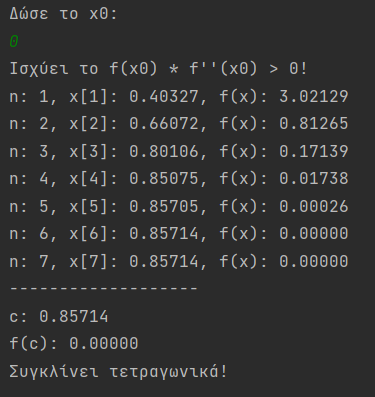
\includegraphics[width=8cm, height=7cm]{images/results_3.png} \end{center}
Όπως βλέπουμε, με αρχικό σημείο \(x_0 = 0\) (για το οποίο ισχύει ο παραπάνω τύπος), χρειάστηκαν πολύ λιγότερες επαναλήψεις για την προσέγγιση της πρώτης ρίζας από την μέθοδο της διχοτόμισης. Επίσης η πρώτη ρίζα συγκλίνει τετραγωνικά αφού ισχύει η συνθήκη:
\[f(c)=0 \text{\hspace{0.3cm}και\hspace{0.3cm}} f'(c)\neq0 \text{\hspace{0.3cm} όπου c η ρίζα της f}\]

\vspace{3mm}

\textbf{Προσοχή!} \\
Αυτό δεν σημαίνει ότι η μέθοδος Newton-Raphson είναι πιο γρήγορη από την μέθοδο της Διχοτόμισης. Δείτε παρακάτω για την επόμενη ρίζα.

\vspace{3mm}
Αποτελέσματα για την δεύτερη ρίζα: \\
\begin{center}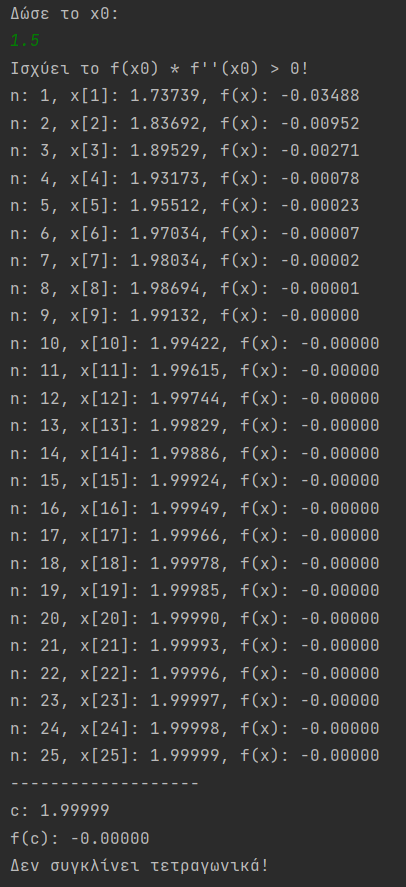
\includegraphics[width=8cm, height=18cm]{images/results_4.png} \end{center}
Όπως βλέπουμε η μέθοδος Newton-Raphson χρειάστηκε 25 επαναλήψεις για την προσσεγιστική εύρεση της 2ης ρίζας με \(x_0 = 1.5\). Αυτό συμβαίνει γιατί η δεύτερη ρίζα και μηδενίζει την πρώτη παράγωγο της f για αυτό και η ρίζα δεν συγκλίνει τετραγωνικά και για αυτό θέλει περισσότερες επαναλήψεις με την μέθοδο Newton-Raphson. \\

Επομένως το χαρακτηριστικό των ριζών που δεν συγκλίνουν τετραγωνικά για την μέθοδο Newton-Raphson είναι ότι μηδενίζουν την πρώτη παράγωγο της συνάρτησης. Πράγμα που κάνει πιο δύσκολη την αναζήτηση της ρίζας αφού η μέθοδος αξιοποιεί την πρώτη παράγωγο ως παρανομαστή κλάσματος.

\subsection{Μέθοδος τέμνουσας: }

Αρχείο κώδικα: "ex 1c.py" \\

Σε περίπτωση που η παράγωγος της συνάρτησης δεν υπάρχει ή δεν μπορεί να υπολογιστεί εύκολα μπορούμε να κάνουμε χρήση της μεθόδου της τέμνουσας αλλάζωντας λίγο τον αναδρομικό τύπο της Newton-Raphson σε:

\[x_{n+1} = x_n - \frac{f(x_n)(x_n - x_{n-1})}{f(x_n) - f(x_{n-1})} , \hspace{0.5cm} n = 1, 2, ...\]

Επομένως χρειαζόμαστε δύο αρχικά σημεία \(x_0, x_1\) για να κάνουμε χρήση του τύπου και με κατάλληλες αρχικοποιήσεις να προσεγγίσουμε τις δύο ρίζες. Η μέθοδος τερματίζει μόλις η απόλυτη τιμή της διαφοράς \(x_{n+1} - x_{n}\) γίνει μικρότερη του σφάλματος ανοχής το οποίο είναι ίσο με \(ε = 10^{(-5)}\)

\pagebreak
Αποτελέσματα για την πρώτη ρίζα: \vspace{3mm} \\
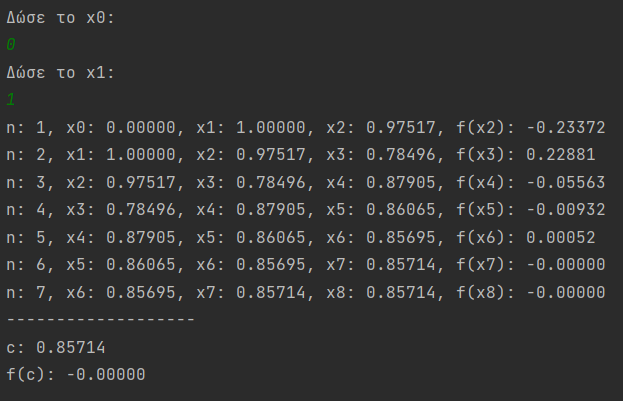
\includegraphics[width=13cm, height=7.5cm]{images/results_5.png} \\

Παρατηρούμε ότι με αρχικά σημεία \(x_0 = 0, x_1 = 1\) η μέθοδος χρειάστηκε 7 επαναλήψεις για να προσεγγίσει την πρώτη ρίζα. \\ 

\pagebreak
Αποτελέσματα για την δεύτερη ρίζα: \vspace{3mm} \\
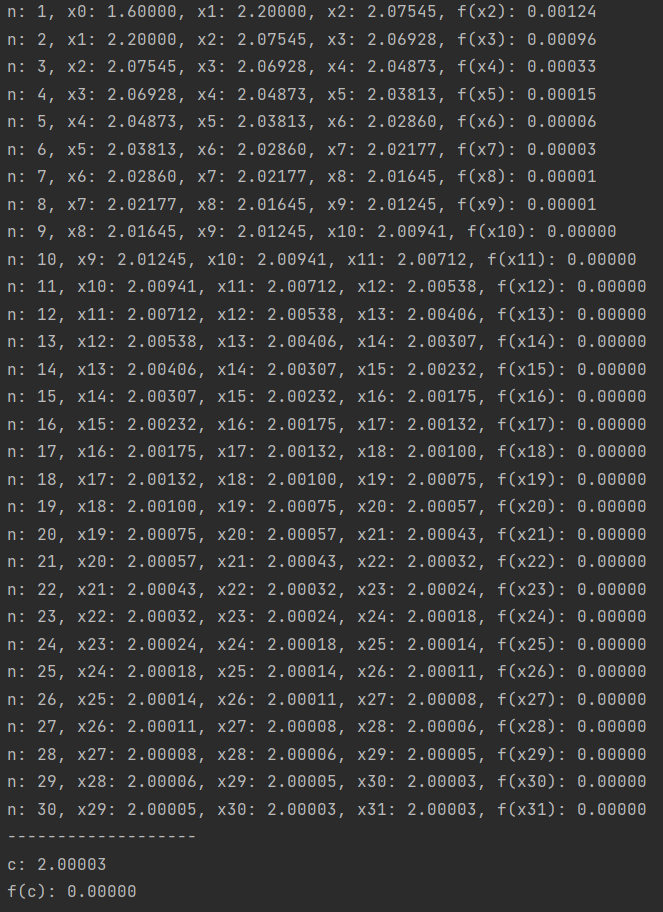
\includegraphics[width=14cm, height=17cm]{images/results_6.png} \\

Παρατηρούμε ότι με αρχικά σημεία \(x_0 = 1.6, x_1 = 2.2\) η μέθοδος χρειάστηκε 30 επαναλήψεις για να προσεγγίσει την δεύτερη ρίζα.

\section{Δεύτερη Άσκηση}

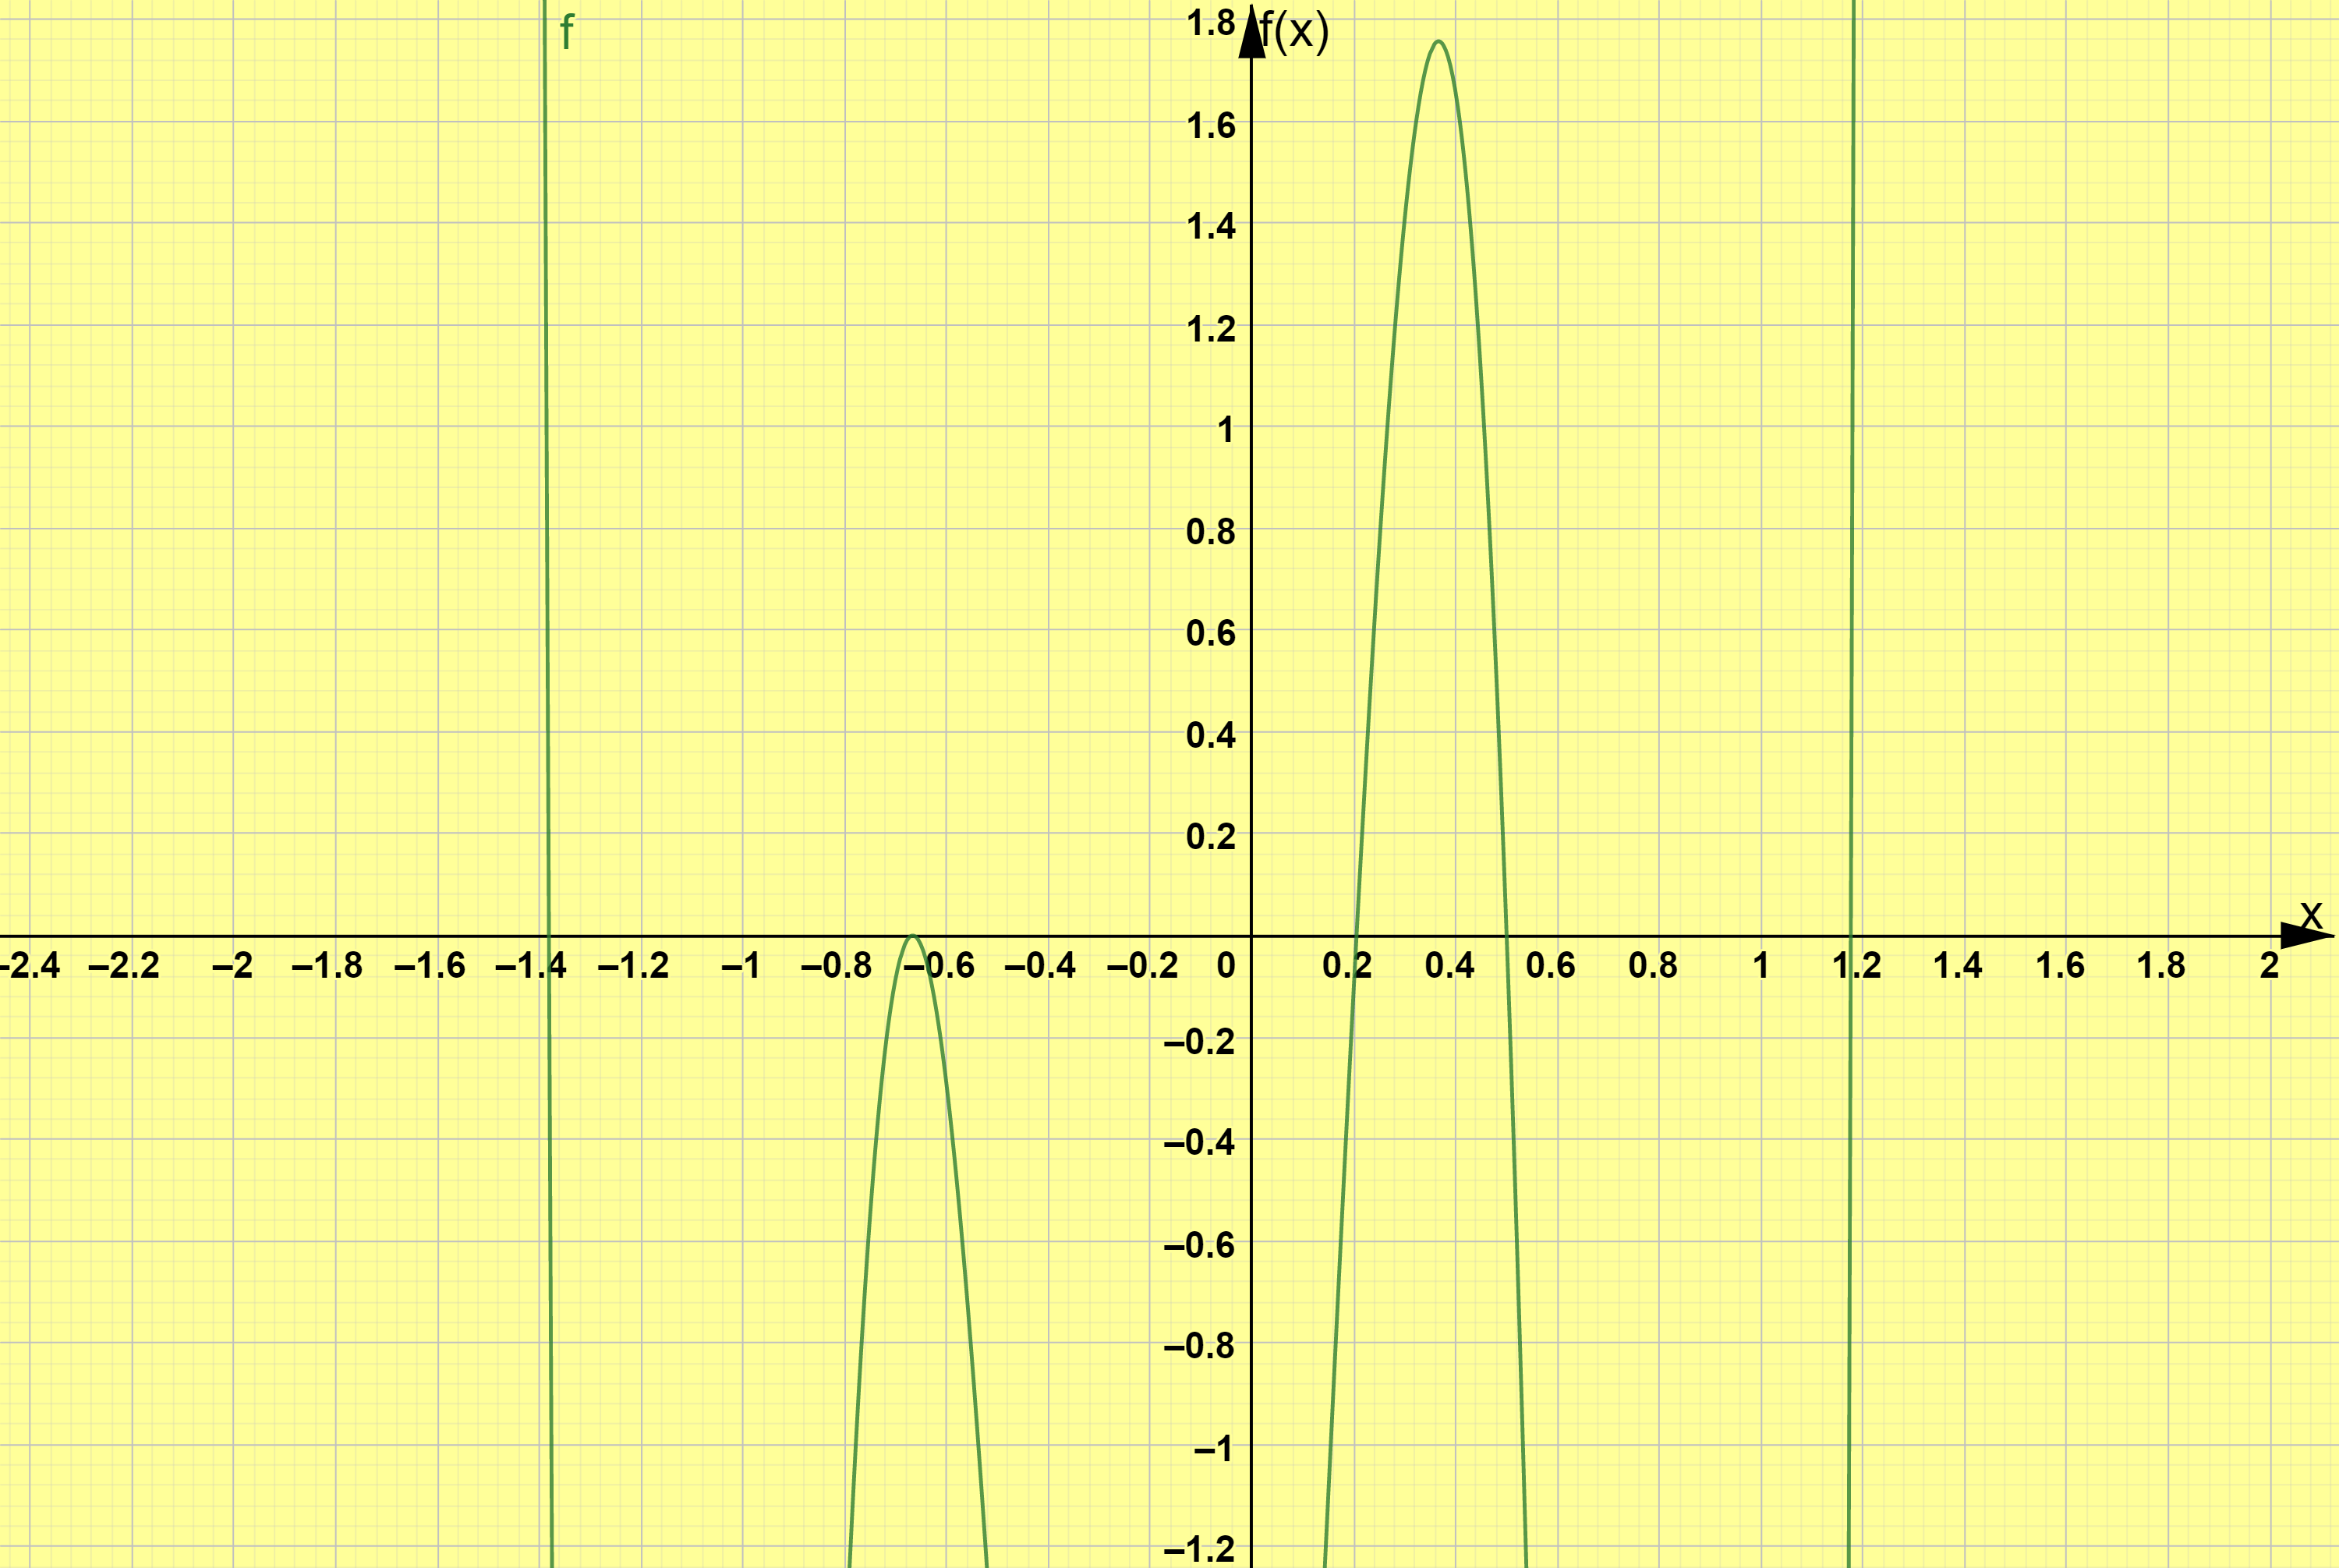
\includegraphics[width=12cm, height=8cm]{images/Figure_2.png} \\
Γραφική παράσταση της συνάρτησης: \(f(x) =  54x^6 + 45x^5 - 102x^4 - 69x^3 + 35x^2 + 16x - 4\)

\vspace{5mm} 
\large{\underline{Μερικά γενικά για την συνάρτηση: }} \\
Όπως παρατηρούμαι η συνάρτηση είναι έκτου βαθμού επομένως περιμένουμε να έχει το πολύ έξι ρίζες. Αρχικά στην γραφική παράσταση φαίνεται να έχουμε 5 ρίζες.

\subsection{Ερώτημα 1:}
    \subsubsection{Τροποποιημένη μέθοδος Newton-Raphson:}
    Αυτό που χρειάζεται να αλλάξουμε στην Newton-Raphson για να έχουμε την νέα τροποποιημένη μέθοδο είναι το όριο h από τον τύπο \(x_{n+1} = x_n = h\) σε: \\
    
    \[h = \frac{1}{\frac{f'(x_n)}{f_(x_n)} - \frac{1}{2}\frac{f''(x_n)}{f'(x_n)}}\]
    
    Η νέα μέθοδος τερματίζει όταν η απόλυτη τιμή του h γίνει μικρότερη του σφάλματος ανοχής \(ε = 10^{(-5)}\). \\
    
    Αποτελέσματα πρώτης ρίζας: \\
    \begin{center}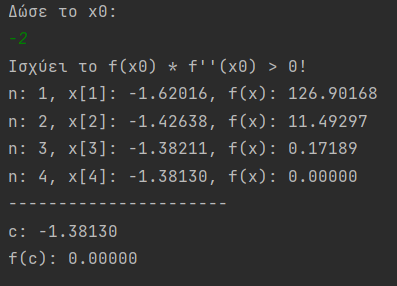
\includegraphics[]{images/results_8.png}\end{center}
    Παρατηρούμε ότι με \(x_0 = -2\) η μέθοδος χρειάστηκε μόνο 4 επαναλήψεις για να βρει την πρώτη ρίζα, δηλαδή την \(c_1 = -1.38130\). 
    
    \vspace{3mm}
    Αποτελέσματα δεύτερης ρίζας: \\
    \begin{center}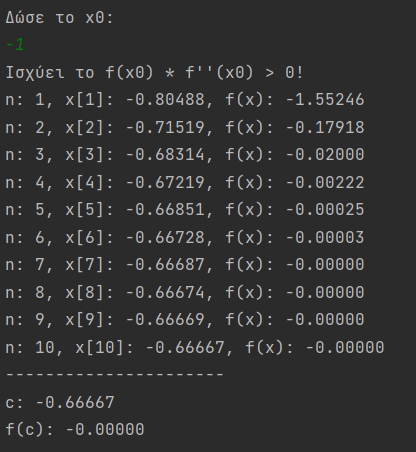
\includegraphics[width = 7cm, height = 7cm]{images/results_9.png}\end{center}
    Παρατηρούμε ότι με \(x_0 = -1\) η μέθοδος χρειάστηκε 10 επαναλήψεις για να βρει την δεύτερη ρίζα, δηλαδή την \(c_2 = -0.66667\).
    
    \vspace{3mm}
    Αποτελέσματα τρίτης ρίζας: \\
    \begin{center}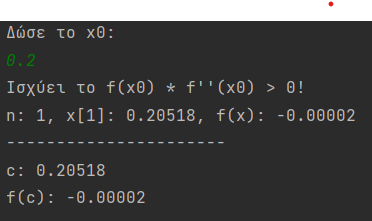
\includegraphics[]{images/results_10.png}\end{center}
    Παρατηρούμε ότι με \(x_0 = 0.2\) η μέθοδος χρειάστηκε μόνο 1 επανάληψη για να βρει την τρίτη ρίζα, δηλαδή την \(c_3 = 0.20518\). 
    
    \vspace{3mm}
    Αποτελέσματα τέταρτης ρίζας: \\
    \begin{center}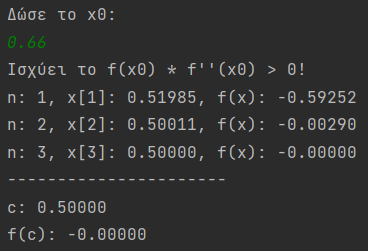
\includegraphics[]{images/results_11.png}\end{center}
    Παρατηρούμε ότι με \(x_0 = 0.66\) η μέθοδος χρειάστηκε μόνο 3 επαναλήψεις για να βρει την τέταρτη ρίζα, δηλαδή την \(c_4 = 0.5\). 
    
    \pagebreak
    \vspace{3mm}
    Αποτελέσματα πέμπτη ρίζας: \\
    \begin{center}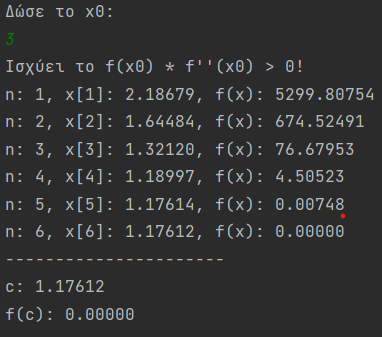
\includegraphics[]{images/results_12.png}\end{center}
    Παρατηρούμε ότι με \(x_0 = 0.3\) η μέθοδος χρειάστηκε 6 επαναλήψεις για να βρει την πέμπτη ρίζα, δηλαδή την \(c_5 = 1.17612\). 
    
    
    \subsubsection{Τροποποιημένη μέθοδος Διχοτόμισης:}
    Το μόνο που χρειάζεται να αλλάξουμε στον κώδικα της μεθόδου της διχοτόμισης για την τροποποίηση είναι την επιλογή του σημείου c από \(c = \frac{a+b}{2}\) όπου πλέον το σημείο επιλέγεται τυχαία μέσω της συνάρτησης uniform(a, b) (από την βιβλιοθήκη random) η οποία επιστρέφει μια τυχαία τιμή από το διάστημα [a, b]. Θα ψάξουμε λοιπόν τις ρίζες ανα διαστήματα.
    
    \pagebreak
    Αποτελέσματα πρώτης ρίζας: \\
    \begin{center}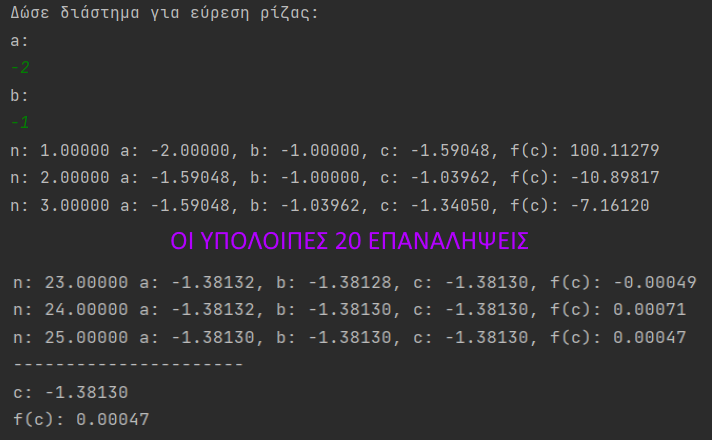
\includegraphics[height = 7cm]{images/results_13.png}\end{center}
    Παρατηρούμε ότι με \(a = -2 \text{και } b = -1\) η μέθοδος χρειάστηκε 25 επαναλήψεις για να βρει την πρώτη ρίζα, δηλαδή την \(c_1 = -1.38130\). 
    
    \vspace{3mm}
    Αποτελέσματα δεύτερης ρίζας: \\
    Επειδή δεν ισχύει το θεώρημα Bolzano στο διάστημα εύρεσης της δεύτερης ρίζας η μέθοδος της διχοτόμισης δεν μπορεί να βρει την δεύτερη ρίζα, δηλαδή την \(c_2 = -0.66667\).
    
    \pagebreak
    \vspace{3mm}
    Αποτελέσματα τρίτης ρίζας: \\
    \begin{center}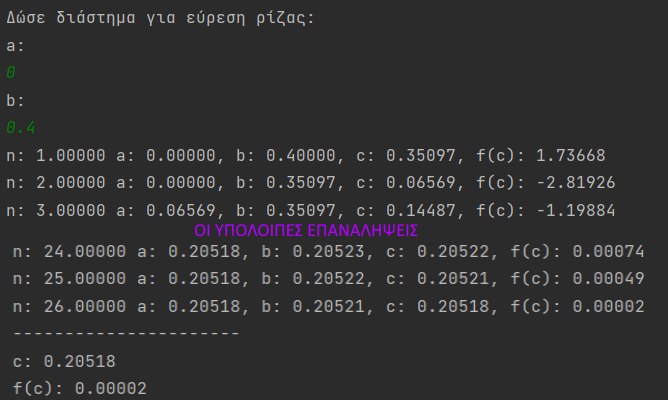
\includegraphics[height = 7cm]{images/results_14.png}\end{center}
    Παρατηρούμε ότι με \(a = 0 \text{και } b = 0.4\) η μέθοδος χρειάστηκε 26 επαναλήψεις για να βρει την τρίτη ρίζα, δηλαδή την \(c_3 = 0.20518\). 
    
    \vspace{3mm}
    Αποτελέσματα τέταρτης ρίζας: \\
    \begin{center}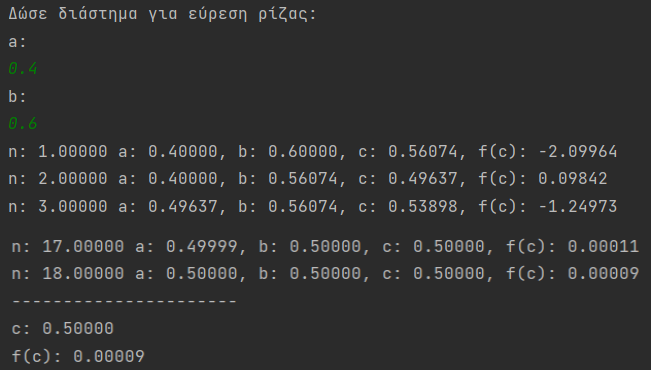
\includegraphics[height = 7cm]{images/results_15.png}\end{center}
    Παρατηρούμε ότι με \(a = 0.4 \text{και } b = 0.6\) η μέθοδος χρειάστηκε 18 επαναλήψεις για να βρει την τέταρτη ρίζα, δηλαδή την \(c_4 = 0.5\).
    
    \vspace{3mm}
    Αποτελέσματα πέμπτη ρίζας: \\
    \begin{center}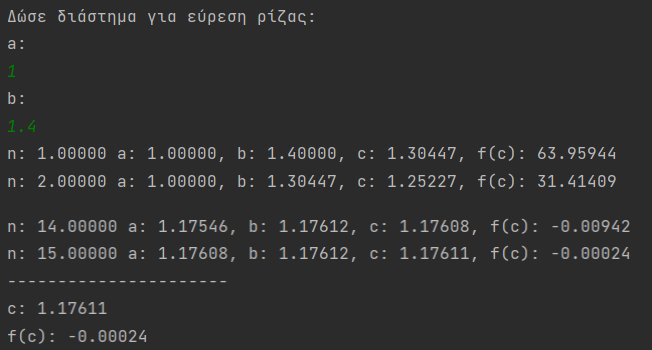
\includegraphics[height = 7cm]{images/results_16.png}\end{center}
    Παρατηρούμε ότι με \(a = 1 \text{και } b = 1.4\) η μέθοδος χρειάστηκε 15 επαναλήψεις για να βρει την πέμπτη ρίζα, δηλαδή την \(c_5 = 1.17612\).
    
    \subsubsection{Τροποποιημένη μέθοδος Τέμνουσας:}
    
    Στην τροποποιημένη μέθοδο της Τέμνουσας απλά αλλάζουμε τον τύπο υπολογισμού του \(x_{n+1}\) αξιοποιώντας τρία αρχικά σημεία. Εδώ θέλει λίγη προσοχή καθώς δεν μπορούμε να δώσουμε το 0 σε αρχικό σημείο γιατί αξιοποιείται στους παρονομαστές των: q, r και s. Η συνθήκη τερματισμού παραμένει ίδια με την κλασσική μέθοδο.
    
    \pagebreak
    Αποτελέσματα πρώτης ρίζας: \\
    \begin{center}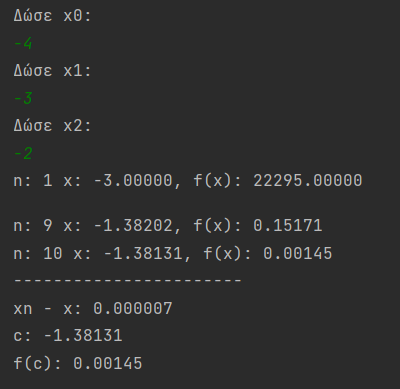
\includegraphics[width = 6cm, height = 6cm]{images/results_17.png}\end{center}
    Παρατηρούμε ότι με \(x_0 = -4 \text{ και } x_1 = -3 \text{ και } x_2 = -2\) η μέθοδος χρειάστηκε 10 επαναλήψεις για να βρει (προσεγγιστικά) την πρώτη ρίζα, δηλαδή την \(c_1 = -1.38130\).
    
    \vspace{3mm}
    Αποτελέσματα δεύτερης ρίζας: \\
    \begin{center}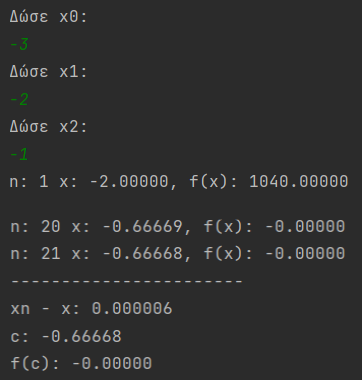
\includegraphics[width = 6cm, height = 6cm]{images/results_18.png}\end{center}
    Παρατηρούμε ότι με \(x_0 = -3 \text{ και } x_1 = -2 \text{ και } x_2 = -1\) η μέθοδος χρειάστηκε 21 επαναλήψεις για να βρει (προσεγγιστικά) την πρώτη ρίζα, δηλαδή την \(c_2 = -0.66667\).
    
    \pagebreak
    \vspace{3mm}
    Αποτελέσματα τρίτης ρίζας: \\
    \begin{center}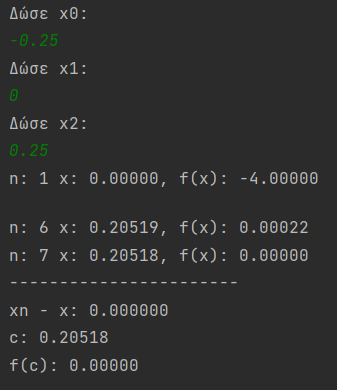
\includegraphics[width = 6cm, height = 6cm]{images/results_19.png}\end{center}
    Παρατηρούμε ότι με \(x_0 = -0.25 \text{ και } x_1 = 0 \text{ και } x_2 = 0.25\) η μέθοδος χρειάστηκε 7 επαναλήψεις για να βρει την πρώτη ρίζα, δηλαδή την \(c_3 = 0.20518\).
    
    \vspace{3mm}
    Αποτελέσματα τέταρτης ρίζας: \\
    \begin{center}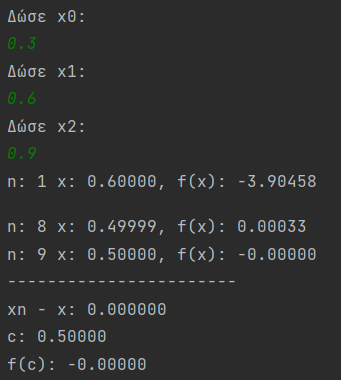
\includegraphics[width = 6cm, height = 6cm]{images/results_20.png}\end{center}
    Παρατηρούμε ότι με \(x_0 = 0.3 \text{ και } x_1 = 0.6 \text{ και } x_2 = 0.9\) η μέθοδος χρειάστηκε 9 επαναλήψεις για να βρει την πρώτη ρίζα, δηλαδή την \(c_4 = 0.5\).
    
    \pagebreak
    \vspace{3mm}
    Αποτελέσματα πέμπτης ρίζας: \\
    \begin{center}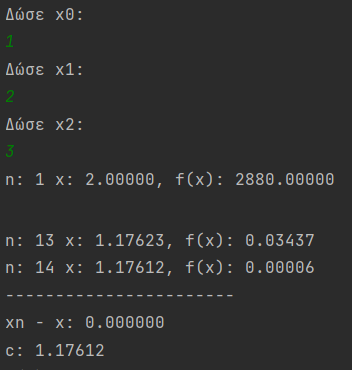
\includegraphics[width = 6cm, height = 6cm]{images/results_21.png}\end{center}
    Παρατηρούμε ότι με \(x_0 = 1 \text{ και } x_1 = 2 \text{ και } x_2 = 3\) η μέθοδος χρειάστηκε 14 επαναλήψεις για να βρει την πρώτη ρίζα, δηλαδή την \(c_5 = 1.17612\).
    
    
\subsection{Ερώτημα 2:}
Τρέχοντας τον αλγόριθμο 10 φορές στο ίδιο διάστημα παρατηρούμε ότι δεν συγκλίνει πάντα στον ίδιο αριθμό επαναλήψεων, που είναι λογικό αφού το σημείο επιλέγεται τυχαία και αυτό σημαίνει ότι μπορεί άλλες φορές να είναι πιο κοντά στην ρίζα, άρα χρειάζονται λιγότερες επαναλήψεις και άλλες φορές πιο μακριά, άρα απαιτούνται περισσότερες επαναλήψεις. \\

Συγκεκριμένα για το διάστημα [0.6, 1.6] της f χρειάστηκαν: 29, 29, 25, 26, 28, 23, 36, 24, 17 και 18 επαναλήψεις για την εύρεση της ρίζας \(x = 1.17611\).

\subsection{Ερώτημα 3:}
Για να συγκρίνουμε τους νέους αλγορίθμους με τους κλασσικούς χρειάζεται να τους χρησιμοποιήσουμε για την ίδια συνάρτηση. Επομένως θα χρησιμοποιήσουμε την συνάρτηση f για τους κλασσικούς αλγορίθμους και θα δούμε πόσο γρήγορα ή όχι συγκλίνουν στην πρώτη ρίζα, δηλαδή την \(c_1 = -1.38130\) με ίδιες αρχικοποιήσεις. \\

    \subsubsection{Κλασσική μέθοδος Newton-Raphson:}
    Αρχείο κώδικα: "ex 2aa.py"
    \begin{center}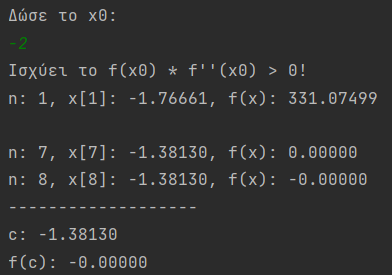
\includegraphics[height = 6cm]{images/results_22.png}\end{center}
    Η κλασσική μέθοδος της Newton-Raphson χρειάστηκε 8 επαναλήψεις για να βρει την ρίζα στο διάστημα με \(x_{0} = -2\). Επομένως μπορούμε να συμπεράνουμε ότι η τροποποιημένη μέθοδος (4 επαναλήψεις με ίδια αρχικοποίηση) είναι πιο γρήγορη από την κλασσική.
        
    \subsubsection{Κλασσική μέθοδος της Διχοτόμισης:}
    Αρχείο κώδικα: "ex 2bb.py"
    \begin{center}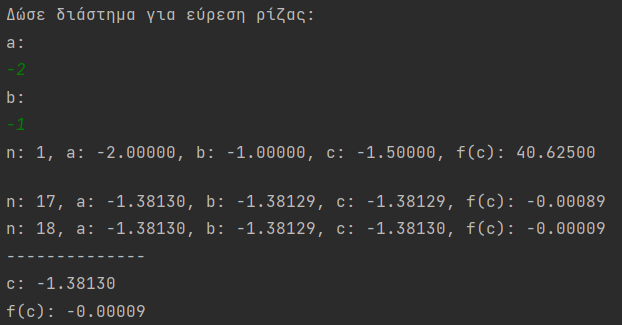
\includegraphics[height = 6cm]{images/results_23.png}\end{center}
    Η κλασσική μέθοδος της διχοτόμισης χρειάστηκε 18 επαναλήψεις για να βρει την ρίζα στο διάστημα [-2, -1]. Αυτό δεν σημαίνει απαραίτητα ότι είναι πιο γρήγορη από την τροποποιημένη μέθοδο καθώς όπως είπανε στο Ερώτημα 2 η νέα μέθοδος χρησιμοποιεί τυχαίο σημείο το οποίο μπορεί είτε να είναι πολύ κοντά στην ρίζα, είτε πολύ μακριά από αυτήν είτε να είναι η ίδια η ρίζα για αυτό και για αυτό μπορεί είτε να αργεί στην σύγκλιση είτε να είναι πολύ πιο γρήγορη από την κλασσική μέθοδο.

    \subsubsection{Κλασσική μέθοδος Tέμνουσας:}
    Αρχείο κώδικα: "ex 2cc.py"
    Με την μέθοδο της Τέμνουσας υπάρχει ένα πρόβλημα. Στην τροποποιημένη χρησιμοποιούμε 3 αρχικά σημεία ενώ στην κλασσική 2. Επομένως θα πάρουμε ως αρχικά της κλασσικής τα δύο τελευταία σημεία που πήραμε στην τροποποιημένη, δηλαδή τα \(x_1 = -3 \text{ και } x_2 = -2\). \\
    \begin{center}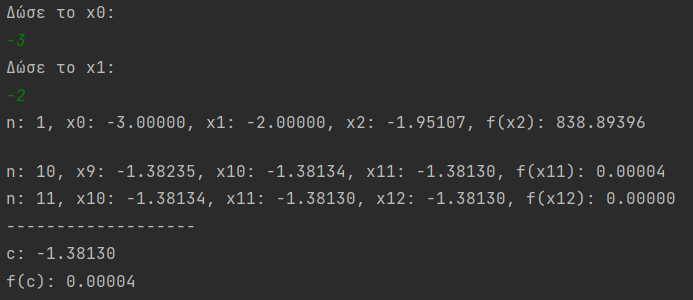
\includegraphics[height = 6cm]{images/results_24.png}\end{center}
    Όπως παρατηρούμε η κλασσική μέθοδος χρειάστηκε 11 επαναλήψεις για να προσεγγίσει την ρίζα. Επομένως μπορούμε να πούμε ότι είναι περίπου όσο γρήγορη είναι η τροποποιημένη.

\pagebreak
\section{Τρίτη Άσκηση}

\subsection{Ερώτημα 1:}

Αρχείο κώδικα: "ex 3a.py" \\

Θα χρησιμοποίησουμε τον παρακάτω 4x4 πίνακα για την \(\textbf{PA = LU}\) παραγοντοποίηση. Ο λόγος που χρησιμοποιούμε τετραγωνικό πίνακα είναι είναι γιατί η \textbf{LU} παραγοντοποίηση παράγει αδύνατο σύστημα για πίνακες nxm με \(n < m\) ενώ για \(n > m\) δεν ορίζεται καν. Ο πίνακας μας λοιπόν είναι ο:

\begin{center}
\textbf{A} =
$\begin{pmatrix}
0 & 2 & -1 & 1\\
-1 & 1 & 2 & -1\\
2 & -1 & 2 & 2\\
1 &  1 & -1 & 2  
\end{pmatrix}$
\end{center}

Ο πίνακας των σταθερών όρων είναι ο:

\begin{center}
\textbf{b} =
$\begin{pmatrix}
6\\
3\\
14\\
8
\end{pmatrix}$
\end{center}

Η συνάρτηση που προγραμματίσαμε επιστρέφει την λύση του της εξίσωσης: \(\textbf{Ax = b}\) κάνοντας χρήση της \(\textbf{PA = LU}\) παραγοντοποίησης. Συγκεκρίμενα, αρχικά ελέγχει αν υπάρχουν μηδενικά στους οδηγούς κάθε σειράς και κάνει αντιμεταθέσεις στον πίνκα \textbf{A} για να δημιουργήσει τον πίνακα \textbf{P} ο οποίος είναι αρχικά ένας μοναδιαίος πίνακας και αλλάζει με τις ίδιες αντιμεταθέσεις σειρών που θα γίνουν στον πίνακα \textbf{A}. Έπειτα χρησιμοποιούμε την μέθοδο Gauss για να λύσουμε την εξίσωση: \(\textbf{LY = Pb}\) όπου \(Y = Ux\). Όπως βλέπουμε αξιοποιούμε τον πίνακα \textbf{P} για να αντιμεταθέσουμε τον πίνακα των σταθερών όρων σε αυτό το σημείο. Στην συνέχεια κάνουμε πάλι Gauss μέθοδο για την εξίσωση \(Ux = Y\) αλλά μόνο κάνωντας αντικαταστάσεις των όρων ανάποδα αφού ο πίνακας \textbf{U} είναι άνω τριγωνικός και επομένως η πρώτη εξάλειψη των κάτω όρων του πίνακα δεν έχει καμία αξία εδώ. Τελικά λαμβάνουμε το διάνυσμα \textbf{x} με τις λύσεις του συστήματος. \\

Τα αποτελέσματα: 
\begin{center}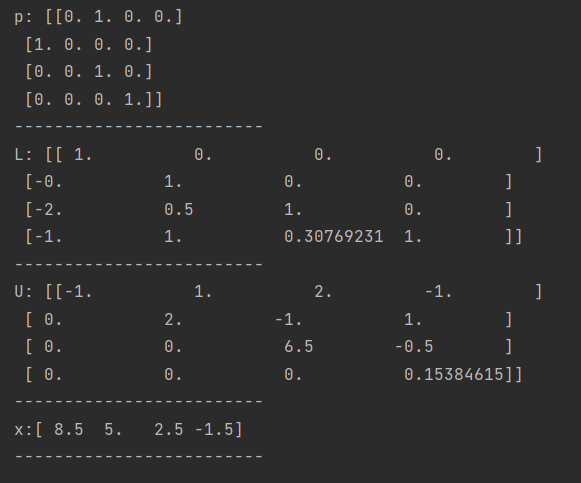
\includegraphics[width = 12cm, height = 10cm]{images/results_27.png}\end{center}

\begin{equation*}
    \textbf{P}  =
    \begin{bmatrix}
        0 & 1 & 0 & 0\\
        1 & 0 & 0 & 0\\
        0 & 0 & 1 & 0\\
        0 & 0 & 0 & 1
    \end{bmatrix} \hspace{0.5cm}
    \textbf{L}  =  
    \begin{bmatrix}
        1 & 0 & 0 & 0\\
        0 & 1 & 0 & 0\\
        -2 & 0.5 & 1 & 0\\
        -1 & 1 & 0.30769231 & 1
    \end{bmatrix} \hspace{0.5cm}
    \textbf{U}  = 
    \begin{bmatrix}
        -1 & 1 & 2 & -1\\
        0 & 2 & -1 & 1\\
        0 & 0 & 6.5 & -0.5\\
        0 & 0 & 0 & 0.15384615
    \end{bmatrix}
\end{equation*}  

\begin{equation*}
    \textbf{x} = 
    \begin{bmatrix}
        8.5\\
        5\\
        2.5\\
        -1.5
    \end{bmatrix}
\end{equation*}

\subsection{Ερώτημα 2:}

Αρχείο κώδικα: "ex 3b.py" \\

Για το ερώτημα αυτό θα χρησιμοποιήσουμε τον συμμετρικό θετικά ορισμένο πίνακα: \\

\begin{center}
\textbf{A} =
$\begin{pmatrix}
2 & 1 & 1\\
1 & 2 & 1\\
1 & 1 & 2
\end{pmatrix}$
\end{center}

Προφανώς είναι συμμετρικός αφού είναι 3x3. Θα αποδείξουμε ότι είναι θετικά ορισμένος. Για να είναι ένας πίνακας θετικά ορισμένος πρέπει όλες οι ιδιοτιμές του είναι θετικές.

\begin{center}
    \begin{equation}
        det(\textbf{A} - λ\textbf{x}) = \begin{vmatrix} 2-λ & 1 & 1\\ 1 & 2-λ & 1\\ 1 & 1 & 2-λ \end{vmatrix} = -(λ-1)^2(λ-4)
    \end{equation}
\end{center}

Από την σχέση (1) παρατηρούμε ότι οι ιδιοτιμές του πίνακα \textbf{Α} είναι λ = 1 (διπλή) και λ = 4, οι οποίες είναι θετικές. Επομένως εδείχθη ότι ο πίνακας \textbf{Α} είναι συμμετρικός και θετικά ορισμένος. \\

Η μέθοδος Cholesky είναι μια επαναληπτική που πάραγει τον κάτω τριγωνικό \textbf{L} πίνακα του Α. Θα χρησιμοποιήσουμε τους παρακάτω τύπους για να υπολογίσουμε τον \textbf{L}:

\begin{center}
    \begin{equation*}
        L_{i,j} = (\pm) \sqrt{A_{j,j} - \sum_{k=1}^{j-1} L^2_{j,k}} \hspace{1cm} \text{αν \(i=j\)}
    \end{equation*}
    \begin{equation*}
        L_{i,j} = \frac{1}{L_{j,j}} (A_{i,j} - \sum_{k=1}^{j-1} L_{i,k}L_{j,k})   \hspace{1cm} \text{αν \(i>j\)}
    \end{equation*}
    \begin{equation*}
        L_{i,j} = 0 \hspace{1cm} \text{αν \(i<j\)}
    \end{equation*}
\end{center}

Επομένως για τον πίνακα \textbf{A} έχουμε: \\
\begin{center}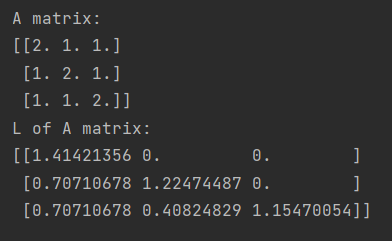
\includegraphics[]{images/results_7.png}\end{center}

\begin{center}
\textbf{L} =
$\begin{pmatrix}
1.41 & 0 & 0\\
0.7 & 1.22 & 0\\
0.7 & 0.4 & 1.15
\end{pmatrix}$
\end{center}


\subsection{Ερώτημα 3:}
Αρχείο κώδικα: "ex 3c.py"

Αρχικά πρέπει να ελέγξουμε αν ισχύει το θεώρημα της σύγκλισης για το σύστημα της εκφώνησης. Παρατηρούμε ότι για κάθε γραμμή εκτός από την πρώτη και την τελευταία ισχύει:

\[|a_{ii}| \geq \sum_{j = 1, j \neq i}^{n}|a_{ij}| \Rightarrow |5| > |-4| \text{\hspace{0.3cm} i = 2, ..., n-1 και j = 1, ..., n}\]
και για τις γραμμές 1 και n
\[|a_{ii}| \geq \sum_{j = 1, j \neq i}^{n}|a_{ij}| \Rightarrow |5| > |-2| \text{\hspace{0.3cm} i = 1 και i = n και j = 1, ..., n}\]

Επομένως μπορούμε να αξιοποιήσουμε την μέθοδο Gauss-Seidel για το σύστημα. Η συνάρτηση στο πρόγραμμα δέχεται 3 πίνακες, τον \textbf{A}, τον \textbf{b} (τους έχουμε αρχικοποιήσει στην αρχή με τις συναρτήσεις filla και fillb) και τον \textbf{x}, ο οποίος στην αρχή είναι ένα μηδενικό διάνυσμα. Έχουμε δυο μεταβλητές στο κύριο πρόγραμμα ώστε να κρατάμε τους δύο τελευταίους πίνακες \textbf{x} και να ελέγχουμε κάθε φορά αν η διαφορά τους ως προς την άπειρη νορμα είναι μικρότερη ή ίση του σφάλματος το οποίο είναι ίσο με 0.00005. Η μέθοδος Gauss-Seidel προσεγγίζει επαναληπτικά την λύση του συστήματος αξιοποιώντας τον παρακάτω τύπο τον οποίο έχουμε υλοποιήσει στην συνάρτηση gauss\_seidel του προγράμματος:

\[x_{i}^{(m+1)} = \frac{1}{a_{ii}} (b_{i} - \sum_{j=1}^{i-1}a_{ij}x_j^{(m+1)} - \sum_{j=i+1}^{n}a_{ij}x_j^{(m)}) \text{\hspace{0.3cm} i = 1, ..., n και m = 1, ...}\]

Τα αποτελέσματα για n = 10: \\
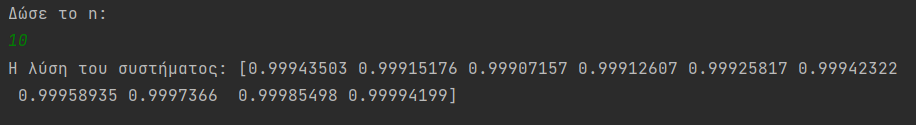
\includegraphics[width = 14cm]{images/results_28.png}
Τα αποτελέσματα για n = 10000: \\
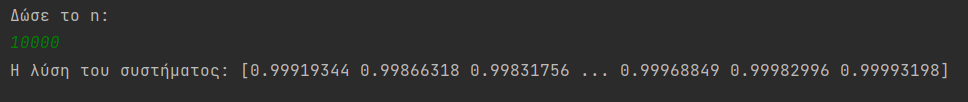
\includegraphics[width = 14cm]{images/results_29.png}


\section{Άσκηση 4:}

Αρχείο κώδικα: "ex 4.py"

Κατασκευάζουμε τον πίνακα G σύμφωνα με την εκφώνηση στις γραμμές 24-29 του αρχείου του κώδικα.

\subsection{Ερώτημα 1:}
Θα χρειαστεί να τρέξουμε μια δομή επανάληψης ώστε να αθροίσουμε κάθε στήλη του πίνακα \textbf{G}, τον οποίο έχουμε ήδη κατασκευάσει, ώστε να δείξουμε ότι όλες οι στήλες έχουν άθροισμα 1, άρα ο πίνακας \textbf{G} θα είναι στοχαστικός. Η δομή βρίσκεται στις γραμμές 31-34 όπου αποθηκεύουμε τα αθροίσματα των στηλών στον πίνακα ni και παρακάτω τον εμφανίζουμε:

\begin{center}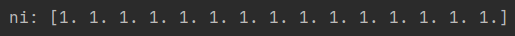
\includegraphics[]{images/results_25.png}\end{center}

Επομένως ο \textbf{G} είναι στοχαστικός.

\subsection{Ερώτημα 2:}

\end{document}